\documentclass[%
	11pt,
	a4paper,
	utf8,
	%twocolumn
		]{article}	

\usepackage{style_packages/podvoyskiy_article_extended}


\begin{document}
\title{Общие и специальные вопросы оптимизации}

\author{\itshape Подвойский А.О.}

\date{}
\maketitle

\thispagestyle{fancy}

%Здесь приводятся заметки по специальным вопросам теории оптимизации


\shorttableofcontents{Краткое содержание}{1}

\tableofcontents

\section{Полезные ссылки}

\url{https://github.com/ceandrade/brkga_mip_feasibility}

\section{Методы решения задач линейного программирования}

\subsection{Симплекс-метод Данцига}

Постановка задачи. Найти максимум функции
\begin{align*}
f(x) = \sum_{j=1}^{n} c_j x_j \leftarrow c^T x
\end{align*}
при ограничениях
\begin{align*}
	\sum_{j=1}^{n} a_{ij} x_j = b_i, \ i = 1, \ldots, m\  (m < n) \leftarrow Ax = b,\\
	x_j \geqslant 0, \ j = 1, \ldots, n.
\end{align*}

Такая постановка называется \emph{канонической}, а искомое решение $ x^{*} = (x_1^{*}, \ldots, x_n^{*})^T $ -- \emph{оптимальным}.

Замечания:
\begin{itemize}
	\item Максимизируемая функция и ограничения \underline{линейны} по $ x_j, \ j = 1, \ldots, n $,
	
	\item Задача содержит ограничения на неотрицательность переменных, присутствие которых диктуется процедурой симплекс-метода. Если по физической постановке задачи какая-либо переменная, например, $ x_n $, неограничена по знаку, то ее можно представить в виде $ x_n = x_{n+1} - x_{n+2} $, где $ x_{n+1}, x_{n+2} \geqslant 0 $,
	
	\item В ограничениях $ \sum\limits_{j=1}^{n} a_{ij} x_j = b_i, \ i = 1, \ldots, m\  (m < n) $ будем считать переменные $ b_i \geqslant 0, \ i = 1, \ldots, m $.
\end{itemize}

Стратегия метода Данцига решения описаной задачи основана на особенностях постановки этой задачи. Множество
\begin{align*}
	X = \{ x \, | \, \sum_{i}^{n} a_{ij} x_j = b_i, \ i = 1, \ldots, m, \ x \in \mathbb{R}^n, \ x_j \geqslant 0, \ j = 1, \ldots, n \}
\end{align*}
допустимых решений задачи -- есть выпуклое множество, которое геометрически представляет собой \emph{выпуклый политоп}\footnote{Политоп -- подмножество Евклидова пространства, представимое объединением симплексов ($ n $-мерное обобщение треугольника)}, имеющий конечное число \emph{крайних точек}.

\emph{Крайней точкой выпуклого множества} $ X $ называется точка $ x \in X $, которая не может быть выражена в виде выпуклой комбинации других точек $ y \in X, x \neq y $.

Стратегия решения задачи симплекс-методом состоит в направленном переборе базисных решений, определяющих крайние точки политопа. Направленность перебора предполагает следующую организацию вычислительного процесса \cite{panteleev}:
\begin{enumerate}
	\item Нахождение базисного решения (метод Гаусса-Жордана, переход к $ M $-задаче),
	
	\item Переход от одного базисного решения к другому таким образом, чтобы обеспечить возрастание целевой функции (другими словами, переход от одной \emph{вершины политопа} к другой в направлении возрастания целевой функции).
\end{enumerate}




\section{Общие положения постановки частично-целочисленного линейного программирования}

Задача линейного программирования в частично-целочисленной постановке (Mixed Integer Linear Program, MILP, MIP) записывается в форме
\begin{align*}
	\min c^T x,\\
	Ax = b,\\
	x \geqslant 0,\\
	x_i \in \mathbb{Z} \quad \forall i \in \mathcal{I}
\end{align*}

Задача, когда все переменные являются целочисленными, называется задачей линейного программирования в чистой целочисленной постановке (Pure Integer Linear Program, ILP, IP).

Если все переменные принимаются значения из множества $ \{ 0, 1 \} $, то задача называется задачей линейного программирования 0-1 (0-1 linear program).

Включение целочисленных переменных в постановку задачи расширяет возможности моделирования.

Задачи линейного программирования могут быть решены за полиномиальное время \emph{методами внутренней точки} (метод эллипсоида, алгоритм Кармаркара). 

Задачи целочисленного программирования относятся к классу NP-трудных:
\begin{itemize}
	\item на текущий момент не известны алгоритмы, способные решить этот такого рода задачи за полиномиальное время,
	
	\item И, вообще говоря, есть мало шансов, что такие алгоритмы когда-нибудь будут найдены.
\end{itemize}

Релаксированное решение можно получить, сняв ограничения на целочисленность
\begin{align*}
	\min c^T x,\\
	Ax = b,\\
	x \geqslant 0.
\end{align*}

\remark{
Задачу линейного программирования в частично-целочисленной постановке нельзя решить, просто перейдя от решения задачи в релаксированной постановке с последующем округлением переменных
}

Например, оптимальным решением задачи линейного программирования в чистой целочисленной постановке будет
\begin{align*}
	\max x + y\\
	-2x + 2 y \geqslant 1,\\
	-8 x + 10 y \leqslant 13,\\
	x,y \geqslant 0,\\
	x,y \in \mathbb{Z}
\end{align*}
вектор $ (x, y) = (1, 2) $, которому отвечает целевая функция со значением 3.

А релаксированным оптимальным решением будет вектор $ (x, y) = (4, 4.5) $ со значением целевой функции 9.5. 

Не существует прямого способа перейти от релаксированного решения к целочисленному.

\begin{figure}[h]
	\centering
	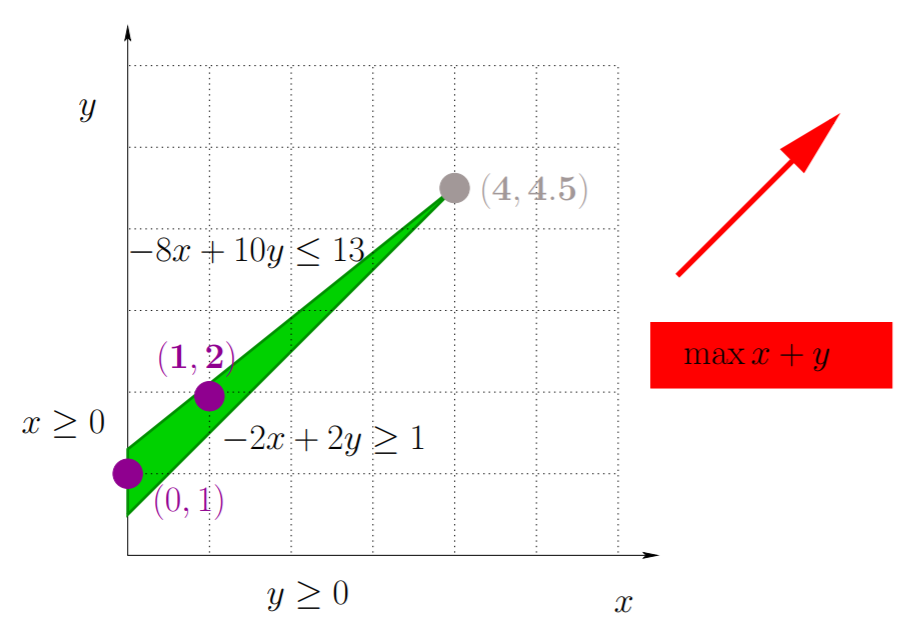
\includegraphics[scale=0.55]{figures/lp_and_mip.png}
	\caption{ Связь релаксированной и целочисленной постановок задачи }\label{fig:lp_and_mip}
\end{figure}

Предполагается, что переменные ограничены, т.е. имеют нижнюю и верхнюю границы.

Через $ P_0 $ обозначим рассматриваемую постановку задачи, а через $ LP(P_0) $ релаксированное решение задачи $ P_0 $. Если в оптимальном релаксированном решении $ LP(P_0) $ все целочисленные переменные принимают целочисленные значения, то это решение будет решением исходной задачи $ P_0 $.

В противном случае для целочисленной переменной $ x_j $, которая принимает нецелочисленное значение $ \beta_j, \ \beta_j \notin \mathbb{Z} $ в оптимальном релаксированном решении $ LP(P_0) $, определяются подзадачи
\begin{align*}
	P_1 := P_0 \wedge x_j \leqslant \floor*{\beta_j},\\
	P_2 := P_0 \wedge x_j \geqslant \ceil*{\beta_j}.
\end{align*}

Тогда физичным решением исходной задачи будет
$$
feasibleSols(P_0) = feasibleSols(P_1) \cup feasibleSols(P_2).
$$



\listoffigures\addcontentsline{toc}{section}{Список иллюстраций}

% Источники в "Газовой промышленности" нумеруются по мере упоминания 
\begin{thebibliography}{99}\addcontentsline{toc}{section}{Список литературы}
	\bibitem{lutz:learningpython-2011}{\emph{Лутц М.} Изучаем Python, 4-е издание. -- Пер. с англ. -- СПб.: Символ-Плюс, 2011. -- 1280~с. }
	
	\bibitem{panteleev}{\emph{Пантлеев}}
	
	\bibitem{burkov:2020}{\emph{Бурков А.} Машинное обучение без лишних слов. -- СПб.: Питер, 2020. -- 192 с.}
		
	\bibitem{beazley:python-2010}{\emph{Бизли Д.} Python. Подробный справочник. -- Пер. с англ. -- СПб.: Символ-Плюс, 2010. -- 864~с. }
\end{thebibliography}

\end{document}
